\small
\begin{figure}[H] 
	\centering
	\includegraphics[scale=0.38]{figures/Cubli-7}
\end{figure}
\begin{figure}[H] 
	\centering
	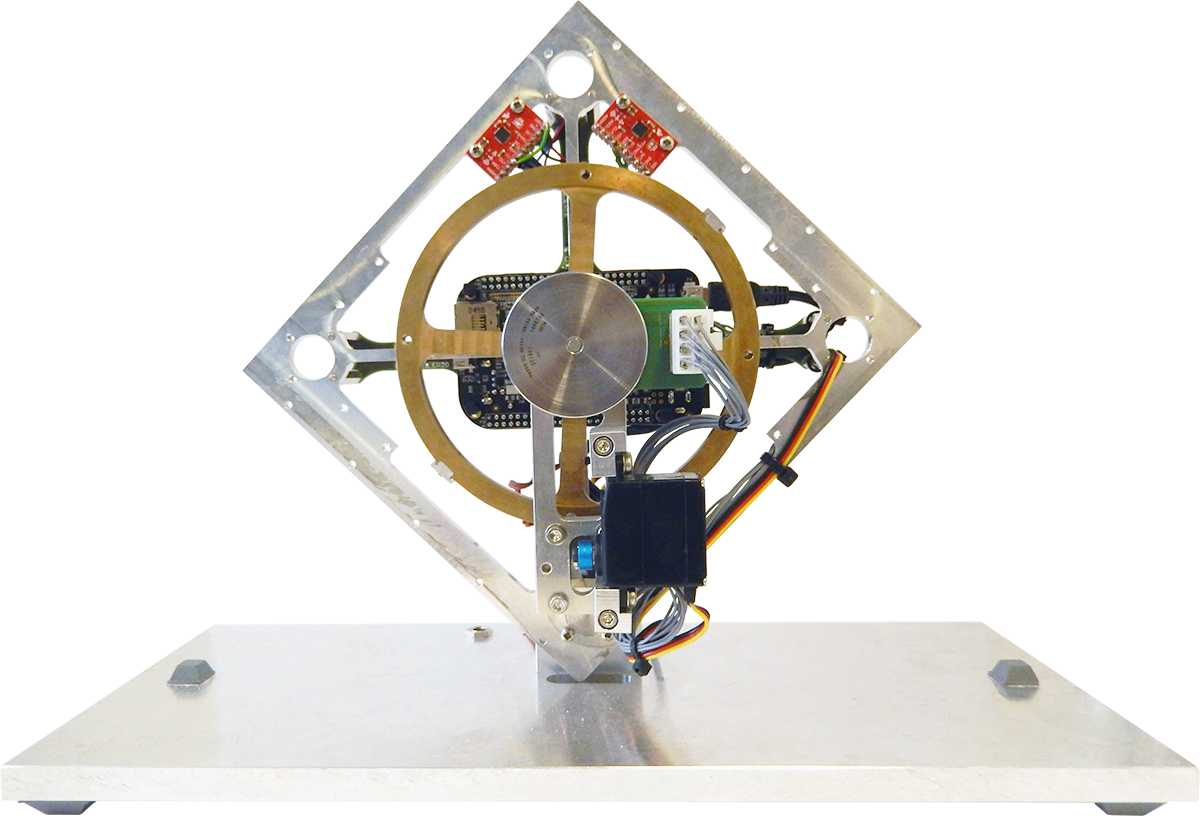
\includegraphics[scale=0.4]{figures/Cubli-2}
\end{figure}
\begin{figure}[H] 
	\centering
	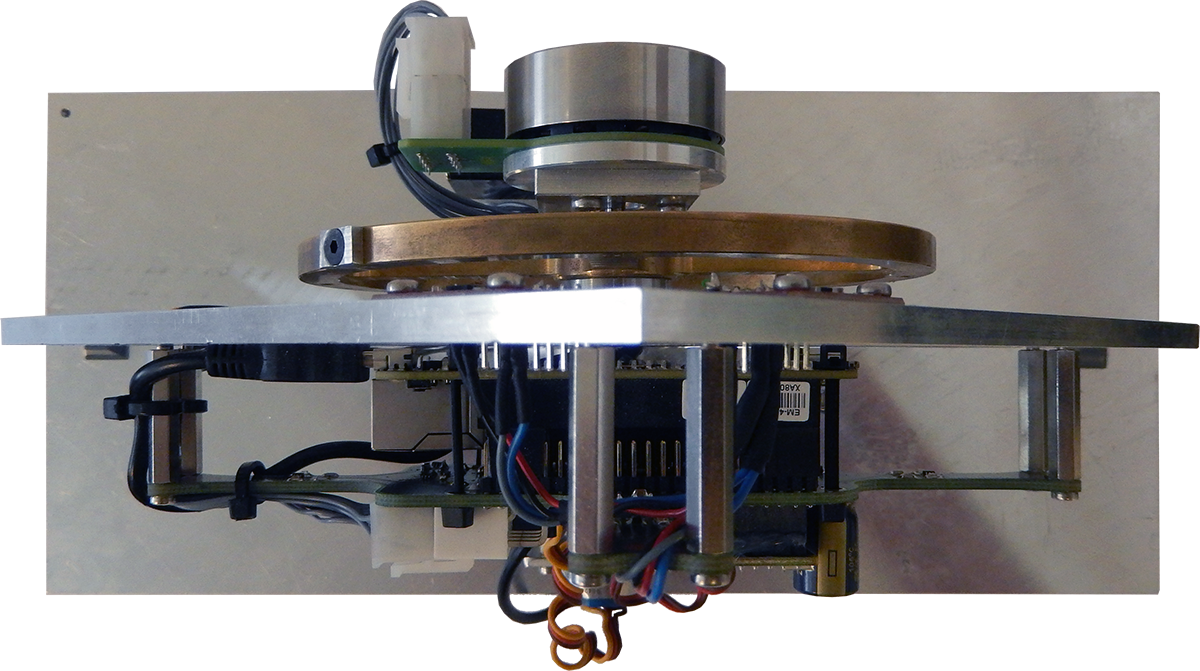
\includegraphics[scale=0.3, angle=180]{figures/Cubli-3}
\end{figure}
\begin{figure}[H] 
	\centering
	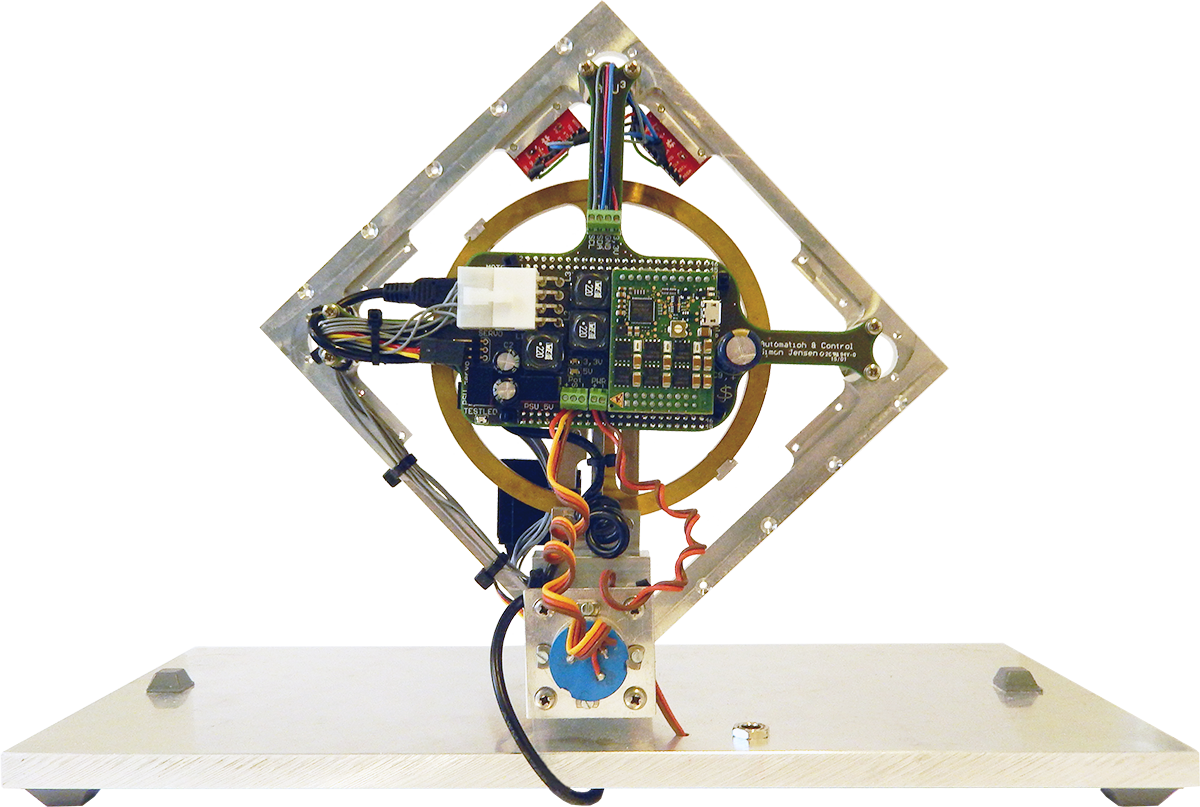
\includegraphics[scale=0.4, angle=180]{figures/Cubli-1}
\end{figure}
\strut\vfill % push the content to the bottom of the page
\noindent Copyright \copyright{} Aalborg University 2016\par
\vspace{0.2cm}

\noindent This report is compiled in \LaTeX, originally developed by Leslie Lamport, based on Donald Knuth's \TeX. The main text is written in \emph{Latin Modern} pt 12, designed by Bogusław Jackowski and Janusz M. Nowacki. 
%The document is compiled via the website \url{www.overleaf.com}, an online collaborative based \LaTeX-editor with instant preview, which enables multiple persons to edit the document simultaneously.
Diagrams are made using Inkscape and Tikz.% Microsoft Visio. 
\clearpage